\documentclass[12pt,letterpaper]{article}
\usepackage{tocloft}
\usepackage[T1]{fontenc}
\usepackage[utf8]{inputenc}
\usepackage[spanish,es-noshorthands]{babel}
\usepackage[margin=2.5cm]{geometry}
\usepackage{graphicx}
\usepackage{mathptmx} % Professional font (Times New Roman style)
\usepackage{amsmath}
\usepackage{amssymb}
\usepackage{longtable}
\usepackage{enumitem}
\usepackage{float}
\usepackage{listings}
\usepackage{caption}
\usepackage{parskip}
\usepackage{tocloft}
\usepackage{svg}
\usepackage{array}
\usepackage{colortbl}
\usepackage{booktabs}
\usepackage[table]{xcolor}
\usepackage{tabularx}


\definecolor{tableheader}{RGB}{238, 237, 232} % Color beige del encabezado
\definecolor{tablerow}{RGB}{249, 249, 247}    % Color beige muy claro para filas intercaladas
\definecolor{stateblue}{RGB}{25, 118, 210}    % Color azul para estados y transiciones

\captionsetup{font=small}

% --- Configuración del Índice (TOC) ---
\setcounter{secnumdepth}{0} % Desactiva la numeración de los títulos en el texto e índice
\setlength{\cftsecnumwidth}{0pt} % Elimina el espacio que ocupaban los números en el índice

% --- Estilo para código / pseudocódigo ---
\lstset{
  basicstyle=\ttfamily\small,
  columns=fullflexible,
  keepspaces=true,
  breaklines=true,
  breakatwhitespace=true,
  frame=single,
  framesep=6pt,
  xleftmargin=6pt,
  xrightmargin=6pt,
  aboveskip=0.8em,
  belowskip=0.8em,
  literate={á}{{\'a}}1 {é}{{\'e}}1 {í}{{\'i}}1 {ó}{{\'o}}1 {ú}{{\'u}}1 {ñ}{{\~n}}1
           {Á}{{\'A}}1 {É}{{\'E}}1 {Í}{{\'I}}1 {Ó}{{\'O}}1 {Ú}{{\'U}}1 {Ñ}{{\~N}}1
}

% --- Macros auxiliares ---
\newcommand{\cd}[1]{\texttt{#1}}                       % lexema / código en línea
\newcommand{\tr}[3]{$#1 \xrightarrow{\,#2\,} #3$}      % transición del autómata
\newcommand{\fin}{^{*}}                                % marca de estado final
\newcommand{\cell}[1]{\parbox[t]{\linewidth}{\raggedright #1}}

\begin{document}

\begin{titlepage}
    \centering
    
    % --- LOGOS AT THE TOP ---
    \begin{minipage}[c]{0.35\textwidth}
        \centering
        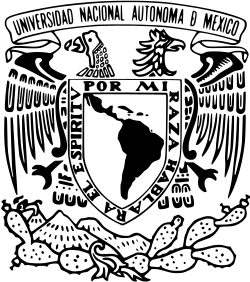
\includegraphics[height=3.5cm]{Escudo-UNAM-escalable.svg.png} % UNAM Logo
    \end{minipage}%
    \hfill
    \begin{minipage}[c]{0.35\textwidth}
        \centering
        
\includegraphics[height=3.5cm]{EscudoFIVectorizadoNegro2008PPNGx5.png} % FI Logo
    \end{minipage}

    \vspace{1cm}

    % --- UNIVERSITY HEADER BELOW LOGOS ---
    {\Large \textbf{UNIVERSIDAD NACIONAL AUTÓNOMA DE MÉXICO}}\\[0.3cm]
    {\large \textbf{FACULTAD DE INGENIERÍA}}\\[0.3cm]
    
    \vfill
    \rule{\linewidth}{1.5pt}\\[0.6cm]

    % --- TITLE & SUBTITLE ---
    {\Large \textbf{LEXICAL ANALYZER}}\\[0.4cm]

    \rule{\linewidth}{1.5pt}
    \vfill

    % --- DETAILS & STUDENT INFO ---
    \begin{flushleft}
        \large
        \textbf{Course:} Compiladores\\[0.2cm]
        \textbf{Group:} 05\\[0.2cm]
        \textbf{Professor:} M.C. René Adrian Dávila Pérez\\[0.2cm]
        \textbf{Student(s):}\\[0.2cm]
        \hspace*{2.8cm} Ambriz Cano Diego Emilio\\[0.2cm]
        \hspace*{2.8cm} Casillas Juárez Camila\\[0.2cm]
        \hspace*{2.8cm} Ferrer Cordero José Manuel\\[0.2cm]
        \hspace*{2.8cm} González Casimiro Juan Carlos\\[0.2cm]
        \hspace*{2.8cm} Vidrio López Mario Alexis\\[0.2cm]
    \end{flushleft}

    \vfill

    % --- LOCATION & DATE ---
    {\large \textbf{Mexico City, \today}}

\end{titlepage}

\newpage
\pagenumbering{arabic} % Comienza la numeración de páginas en 1
\tableofcontents
\newpage

% --- CONTENIDO DEL DOCUMENTO ---

%=====================================================================
\section{Introducción}

En este documento se presentan las decisiones de modelado utilizadas para definir el comportamiento del analizador léxico, así como los elementos que posteriormente servirán como base para su implementación.

\textbf{Qué se hizo.} Una definición regular por cada clase de token y por cada elemento que se descarta.

\begin{align*}
\text{letra} &\rightarrow [\text{a-zA-Z}] \\
\text{digito} &\rightarrow [0\text{-}9] \\
\text{escape} &\rightarrow \backslash\ (\text{cualquier carácter excepto salto de línea}) \\
\text{identificador} &\rightarrow (\text{letra} \mid \text{\_})\ (\text{letra} \mid \text{digito} \mid \text{\_})^* \\
\text{reservada} &\rightarrow \text{un lexema de identificador que está en la tabla de búsqueda} \\
\text{entero} &\rightarrow \text{digito}^+ \\
\text{decimal} &\rightarrow \text{digito}^+\ .\ \text{digito}^+ \\
\text{caracter} &\rightarrow \text{\textquotesingle}\ (\text{cualquier carácter excepto \textquotesingle, } \backslash \text{ y salto de línea} \mid \text{escape})\ \text{\textquotesingle} \\
\text{booleano} &\rightarrow \text{true} \mid \text{false} \quad \text{(se reconoce como identificador y se busca en la tabla)} \\
\text{constante} &\rightarrow \text{entero} \mid \text{decimal} \mid \text{caracter} \mid \text{booleano} \\
\text{literal} &\rightarrow \text{\textquotedbl}\ (\text{cualquier carácter excepto \textquotedbl, } \backslash \text{ y salto de línea} \mid \text{escape})^*\ \text{\textquotedbl} \\
\text{operador} &\rightarrow + \mid - \mid * \mid / \mid \% \mid = \mid == \mid ! \mid != \mid < \mid <= \mid > \mid >= \mid \& \mid \&\& \mid \text{\textquotedbl}\!\mid\!\text{\textquotedbl} \mid \text{\textquotedbl}\!\mid\!\mid\!\text{\textquotedbl} \\
\text{puntuacion} &\rightarrow ( \mid ) \mid \{ \mid \} \mid [ \mid ] \mid ; \mid , \\
\text{especial} &\rightarrow \# \mid . \\
\text{blanco} &\rightarrow (\text{espacio} \mid \backslash\text{t} \mid \backslash\text{r} \mid \backslash\text{n})^+ \quad \text{se descarta} \\
\text{comentario} &\rightarrow // \ (\text{cualquier carácter excepto salto de línea})^* \\
&\quad \mid /* \ ([\hat{\ }*] \mid *^+ [\hat{\ }*/])^* \ *^+ / \quad \text{se descarta}
\end{align*}

Para los identificadores se consideró que el primer carácter puede ser una letra o guion bajo, mientras que los siguientes pueden incluir letras, dígitos o guion bajo. El decimal exige al menos un dígito después del punto, así que "5." no es una constante completa.

Los signos + y - no se consideran parte de las constantes numéricas, sino operadores independientes. De esta manera, una expresión como a-1 se reconoce como un identificador, un operador de resta y una constante entera.

El token del tipo “scape” "(símbolo \textbackslash)~" se aplica en cadenas y constantes, su uso permite al Lexer agregar comillas u otros caracteres distintos al salto de línea a cadenas de texto sin la interpretación de fin de cadena. Por ejemplo, en \texttt{"Hello \textbackslash"John\textbackslash""}, la comilla seguida del símbolo definido como scape no implica el final de la cadena.

Los tokens del tipo "Literal y Caracter" no admiten saltos de línea, en consecuencia, el analizador detecta un error en la línea donde empiezan la cadena si esta no se cierra correctamente. Las literales se refieren a las cadenas construidas entre comillas dobles, "...", mientras que los caracteres son constantes que contienen exactamente solo un elemento entre comillas simples ' '.

Los tokens de tipo boolean (true y false) son palabras, estas siguen el camino del identificador y se distinguen en la tabla de búsqueda; no necesitan estados propios. En los comentarios de bloque se permite cualquier contenido hasta encontrar la secuencia de cierre */. El patrón debe evitar que un asterisco aislado cierre el comentario de forma incorrecta.

El analizador lee todo el lexema hasta generar un token válido, aún si encuentra caracteres o identificadores catalogados a cierto token específico, se lee por completo.Al finalizar se compara con alguna de las palabras u operadores reservados.

Estas expresiones regulares sirven como base para la construcción de los autómatas. En la implementación no se van a usar directamente mediante una biblioteca de expresiones regulares, ya que serán representadas mediante el AFD que se va a construir más adelante.

%=====================================================================
\section{Definición formal de cada token}

A continuación se presenta una lista de 45 tokens agrupados en Palabra reservada, identificador, constante, literal, operador, puntuación y carácter especial.

\begin{center}
\small
\begin{longtable}{@{}r l l p{6.6cm}@{}}
\toprule
\textbf{\#} & \textbf{TokenType} & \textbf{Clase (salida)} & \textbf{Lexema o patrón} \\
\midrule
\endhead
\bottomrule
\endfoot
1  & \cd{INT}         & keyword     & \cd{int} \\
2  & \cd{FLOAT}       & keyword     & \cd{float} \\
3  & \cd{CHAR}        & keyword     & \cd{char} \\
4  & \cd{DOUBLE}      & keyword     & \cd{double} \\
5  & \cd{VOID}        & keyword     & \cd{void} \\
6  & \cd{RETURN}      & keyword     & \cd{return} \\
7  & \cd{IF}          & keyword     & \cd{if} \\
8  & \cd{ELSE}        & keyword     & \cd{else} \\
9  & \cd{WHILE}       & keyword     & \cd{while} \\
10 & \cd{FOR}         & keyword     & \cd{for} \\
11 & \cd{PRINT}       & keyword     & \cd{print} \\
12 & \cd{ID}          & identifier  & \cd{letra} \\ 
13 & \cd{INT\_CONST}  & constant    & \cd{uno o más digitos} \\
14 & \cd{FLOAT\_CONST}& constant    & dígitos, punto, dígitos \\
15 & \cd{CHAR\_CONST} & constant    & un carácter o un escape entre comillas simples \\
16 & \cd{TRUE}        & constant    & \cd{true} \\
17 & \cd{FALSE}       & constant    & \cd{false} \\
18 & \cd{STRING}      & literal     & cero o más caracteres o escapes entre comillas dobles \\
19 & \cd{PLUS}        & operator    & \cd{+} \\
20 & \cd{MINUS}       & operator    & \cd{-} \\
21 & \cd{STAR}        & operator    & \cd{*} \\
22 & \cd{SLASH}       & operator    & \cd{/} \\
23 & \cd{PERCENT}     & operator    & \cd{\%} \\
24 & \cd{ASSIGN}      & operator    & \cd{=} \\
25 & \cd{EQ}          & operator    & \cd{==} \\
26 & \cd{NOT}         & operator    & \cd{!} \\
27 & \cd{NEQ}         & operator    & \cd{!=} \\
28 & \cd{LT}          & operator    & \cd{<} \\
29 & \cd{LE}          & operator    & \cd{<=} \\
30 & \cd{GT}          & operator    & \cd{>} \\
31 & \cd{GE}          & operator    & \cd{>=} \\
32 & \cd{AMP}         & operator    & \cd{\&} \\
33 & \cd{AND}         & operator    & \cd{\&\&} \\
34 & \cd{BAR}         & operator    & \cd{\textbar} \\
35 & \cd{OR}          & operator    & \cd{\textbar\textbar} \\
36 & \cd{LPAREN}      & punctuation & \cd{(} \\
37 & \cd{RPAREN}      & punctuation & \cd{)} \\
38 & \cd{LBRACE}      & punctuation & \cd{\{} \\
39 & \cd{RBRACE}      & punctuation & \cd{\}} \\
40 & \cd{LBRACKET}    & punctuation & \cd{[} \\
41 & \cd{RBRACKET}    & punctuation & \cd{]} \\
42 & \cd{SEMI}        & punctuation & \cd{;} \\
43 & \cd{COMMA}       & punctuation & \cd{,} \\
44 & \cd{HASH}        & special     & \cd{\#} \\
45 & \cd{DOT}         & special     & \cd{.} \\
\end{longtable}
\end{center}

%=====================================================================
\subsection{Prioridad de reconocimiento}
La prioridad de los Tokens, cuando se reconoce más de un padrón a la entrada, se determinó a partir de las siguientes cinco reglas.

\begin{enumerate}
    \item \textbf{Máximo bocado.} Toma el lexema más largo que termine en un estado final.
    \item \textbf{Tabla antes que identificador.} Si el lexema termina en $q_1$ y está en la tabla de búsqueda, gana la tabla. Por ejemplo: \cd{int} es palabra reservada y \cd{true} es constante.
    \item \textbf{Lo que no es token compite igual.} Espacios y comentarios se reconocen con las mismas reglas y después se descartan.
    \item \textbf{Excepción del comentario sin cerrar.} Si la entrada se acaba dentro de un comentario de bloque ($q_{10}$ o $q_{11}$), no se retrocede al \cd{/} de $q_8$: se reporta comentario sin cerrar.
    \item \textbf{Sin estado final no hay token.} Si ningún prefijo llega a un estado final, se reporta un error léxico; no existe un token por defecto.
\end{enumerate}

El máximo bocado es el primero porque toma la decisón en la mayoría de los casos y \textbf{nunca entra en conflicto con las otras reglas}. La tabla va después porque solo actúa cuando el lexema ya terminó en $q_1$. Con estas reglas se resuelven los casos de ambigüedad considerados en el lenguaje definido para la práctica.

 La regla cuatro se presenta en el AFD. Si \cd{/* ...} llega al final sin cerrarse, el último estado final visitado es $q_8$; sin la excepción, el escáner retrocedería y reportaría un operador \cd{/} en vez del error real.

%=====================================================================
\section{AFND}

El siguiente autómata fue realizado en colaboración con los compañeros de clase durante una de de las sesiones teóricas de la materia. Este sirve como base teórica para la construcción del autómata correspondiente a analizador léxico de este proyecto.

\begin{figure}[H]
    \centering
    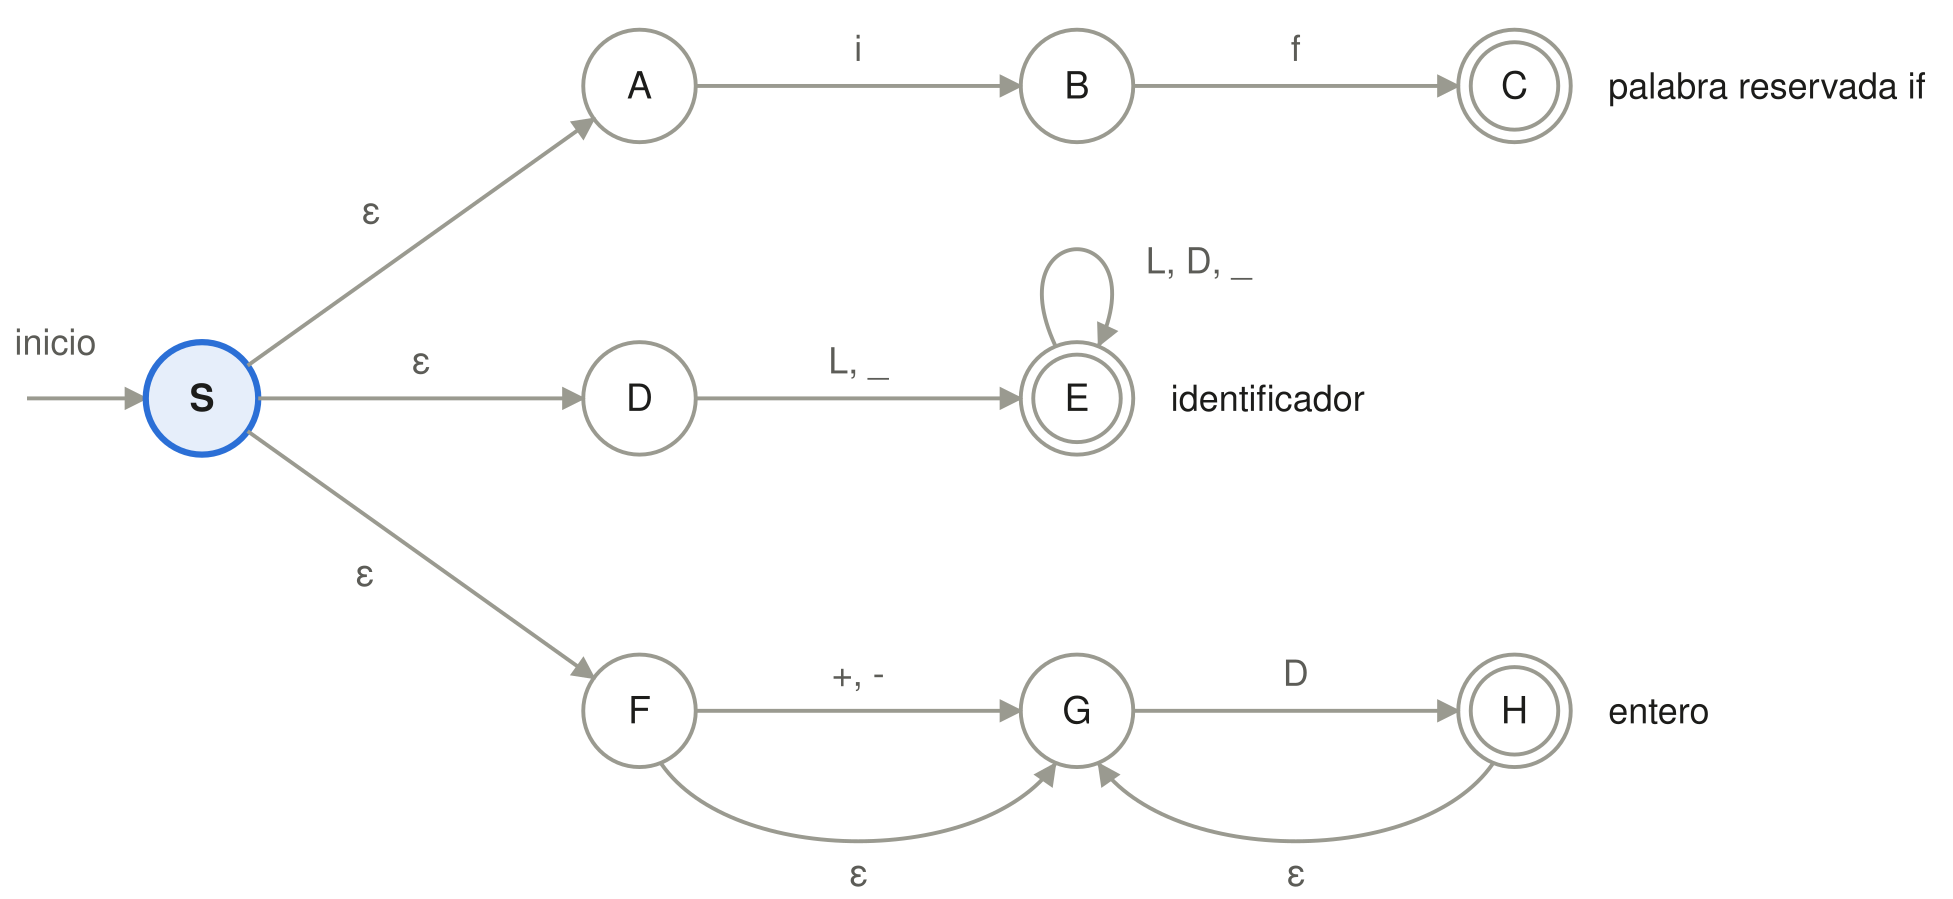
\includegraphics[width=0.95\textwidth]{afnd-ejemplo.png}
    \caption{AFD realizado en sesiones teóricas.}
\end{figure}

\begin{flushleft}
\begin{tabular}{@{}p{0.62\textwidth} l@{}}
\tr{S}{\varepsilon}{A}\quad \tr{S}{\varepsilon}{D}\quad \tr{S}{\varepsilon}{F} & \\[0.3em]
\tr{A}{\cd{i}}{B}\quad \tr{B}{\cd{f}}{C\fin} & palabra reservada \cd{if} \\[0.3em]
\tr{D}{\cd{[a-zA-Z\_]}}{E\fin}\quad \tr{E}{\cd{[a-zA-Z0-9\_]}}{E} & identificador \\[0.3em]
\tr{F}{\cd{+}|\cd{-}}{G}\quad \tr{F}{\varepsilon}{G}\quad \tr{G}{\cd{[0-9]}}{H\fin}\quad \tr{H}{\varepsilon}{G} & entero \\
\end{tabular}

\smallskip
$(^{*} = \text{estado final})$
\end{flushleft}

\subsection{AFND. Lexical Analyzer}

Cada definición regular de la sección 1 se tradujo a un sub-autómata, es decir, un estado por cada punto del patrón donde se espera un tipo distinto de carácter, y un estado final donde el patrón puede terminar. Después, S se unió a los nueve estados iniciales del autómata de la sección anterior con movimientos $\varepsilon$.

\vspace{0.3cm}

{\small
\noindent
\rowcolors{2}{tablerow}{white}
\begin{tabularx}{\textwidth}{@{} >{\bfseries}p{2.8cm} X p{5.5cm} @{}}
\rowcolor{tableheader}
\textbf{Sub-autómata} & \textbf{Transiciones (origen $\rightarrow$ símbolo $\rightarrow$ destino)} & \textbf{Estados finales} \\ 
\toprule

Inicio & $S \xrightarrow{\,\varepsilon\,} I_0, N_0, T_0, K_0, C_0, O_0, P_0, X_0, W_0$ & $S$: estado inicial \\

Identificador & $I_0 \xrightarrow{\,L\,} I_1^*$ \quad $I_1 \xrightarrow{\,L \mid D\,} I_1^*$ & $I_1$: identificador o reservada \\

Número & $N_0 \xrightarrow{\,D\,} N_1^*$ \quad $N_1 \xrightarrow{\,D\,} N_1^*$ \quad $N_1 \xrightarrow{\,.\,} N_2$ & $N_1$: entero \\
& $N_2 \xrightarrow{\,D\,} N_3^*$ \quad $N_3 \xrightarrow{\,D\,} N_3^*$ & $N_3$: decimal \\

Cadena & $T_0 \xrightarrow{\,"\,} T_1$ \quad $T_1 \xrightarrow{\,c\,} T_1$ \quad $T_1 \xrightarrow{\,\backslash\,} T_2$ & $T_3$: literal (cadena) \\
& $T_2 \xrightarrow{\,a\,} T_1$ \quad $T_1 \xrightarrow{\,"\,} T_3^*$ & \\

Carácter & $K_0 \xrightarrow{\,'\,} K_1$ \quad $K_1 \xrightarrow{\,k\,} K_2$ \quad $K_1 \xrightarrow{\,\backslash\,} K_3$ & $K_4$: constante de carácter \\
& $K_3 \xrightarrow{\,a\,} K_2$ \quad $K_2 \xrightarrow{\,'\,} K_4^*$ & \\

Comentarios & $C_0 \xrightarrow{\,/\,} C_1$ \quad $C_1 \xrightarrow{\,/\,} C_2^*$ \quad $C_2 \xrightarrow{\,a\,} C_2^*$ & $C_2$: comentario de línea \\
& $C_1 \xrightarrow{\,*\,} C_3$ \quad $C_3 \xrightarrow{\,m\,} C_3$ \quad $C_3 \xrightarrow{\,*\,} C_4$ & $C_5$: comentario de bloque \\
& $C_4 \xrightarrow{\,*\,} C_4$ \quad $C_4 \xrightarrow{\,n\,} C_3$ \quad $C_4 \xrightarrow{\,/\,} C_5^*$ & (ambos se descartan) \\

Operadores & $O_0 \xrightarrow{\text{+ - * \% /}} O_1^*$ \quad $O_0 \xrightarrow{\text{= ! < >}} O_2^*$ \quad $O_2 \xrightarrow{\text{=}} O_3^*$ & $O_1, O_2, O_4, O_5$: un carácter \\
& $O_0 \xrightarrow{\text{\&}} O_4^*$ \quad $O_4 \xrightarrow{\text{\&}} O_3^*$ \quad $O_0 \xrightarrow{\text{|}} O_5^*$ & $O_3$: dos caracteres \\
& $O_5 \xrightarrow{\text{|}} O_3^*$ & \\

Puntuación & $P_0 \xrightarrow{\,\text{PUNCT}\,} P_1^*$ & $P_1$: puntuación \\

Especial & $X_0 \xrightarrow{\,\#\, .\,} X_1^*$ & $X_1$: carácter especial \\

Blanco & $W_0 \xrightarrow{\,\text{WS, NL}\,} W_1^*$ \quad $W_1 \xrightarrow{\,\text{WS, NL}\,} W_1^*$ & $W_1$: blanco (se descarta) \\
\bottomrule
\end{tabularx}
}

\vspace{0.4cm}

\textbf{Símbolos}
{\small
\begin{flushleft}
\begin{tabular}{@{}l l l l@{}}
$L$ = letra o \_ & $D$ = dígito & $\text{PUNCT} = \cd{( ) \{ \} [ ] ; ,}$ & $\text{WS} = \text{espacio, tabulador, CR}$ \\
$c$ = cualquier carácter excepto \cd{"}, \cd{\textbackslash} y NL & $k$ = cualquier carácter excepto \cd{\textquotesingle}, \cd{\textbackslash} y NL & $a$ = cualquier carácter excepto NL & $\text{NL} = \text{salto de línea}$ \\
$m$ = cualquier carácter excepto \cd{*} & $n$ = cualquier carácter excepto \cd{*} y \cd{/} & $[\ ] = \text{cualquiera de los símbolos indicados}$ & \\
\end{tabular}
\end{flushleft}
}

Único no determinismo: $S$, que con $\varepsilon$ abre los nueve sub-autómatas a la vez, y el carácter \cd{/}, que lleva tanto a $O_1$ (operador) como a $C_1$ (comentario). Cada sub-autómata, por separado, ya es determinista.


%=====================================================================
\section{Conversión AFND $\rightarrow$ AFD}

Un AFD tiene exactamente un movimiento por estado y símbolo, así que se ejecuta en una sola pasada con una consulta a la tabla por carácter. El AFD resultante puede implementarse mediante una tabla de transiciones, permitiendo determinar el siguiente estado a partir del estado actual y la clase del carácter leído.

\subsection{Método, con el ejemplo de clase}

Se usan dos operaciones. $\varepsilon$-cerradura($T$) son los estados a los que se llega desde $T$ solo con $\varepsilon$; mover($T$, $a$) son los estados a los que se llega desde $T$ con el símbolo $a$. Cada estado del AFD es un conjunto de estados del AFND.

\begin{enumerate}
    \item $Q_0 = \varepsilon\text{-cerradura}(S)$. Desde $S$, $\varepsilon$ lleva a $A$, $D$ y $F$; desde $F$, $\varepsilon$ lleva a $G$. $Q_0 = \{S, A, D, F, G\}$.
    \item Desde $Q_0$ con \cd{i}: $A$ pasa a $B$ y $D$ pasa a $E$. Resultado $\{B, E\} = Q_1$.
    \item Desde $Q_0$ con \cd{f}, otra letra o \cd{\_}: solo $D$ se mueve, a $E$. Resultado $\{E\} = Q_2$.
    \item Desde $Q_0$ con un dígito: $G$ pasa a $H$, y por $\varepsilon$ $H$ regresa a $G$. Resultado $\{G, H\} = Q_3$.
    \item Desde $Q_0$ con \cd{+} o \cd{-}: $F$ pasa a $G$. Resultado $\{G\} = Q_4$.
    \item Desde $Q_1$ con \cd{f}: $B$ pasa a $C$ y $E$ se queda en $E$. Resultado $\{C, E\} = Q_5$.
    \item Desde $Q_1$ con otra letra o un dígito: solo $E$ se mueve. Resultado $\{E\} = Q_2$.
    \item $Q_2$ se cicla en sí mismo; $Q_3$ y $Q_4$ con dígito van a $Q_3$; $Q_5$ con letra o dígito va a $Q_2$ (\cd{ifx} es identificador).
    \item Un estado del AFD es final si contiene algún estado final del AFND.
\end{enumerate}

\begin{center}
\small
\begin{tabularx}{\textwidth}{@{}l l c c c c c X@{}}
\toprule
\textbf{Estado AFD} & \textbf{Estados AFND} & \cd{i} & \cd{f} & \textbf{otra letra, \cd{\_}} & \textbf{dígito} & \cd{+} o \cd{-} & \textbf{¿Final?} \\
\midrule
$Q_0$ & $\{S, A, D, F, G\}$ & $Q_1$ & $Q_2$ & $Q_2$ & $Q_3$ & $Q_4$ & no \\
$Q_1$ & $\{B, E\}$ & $Q_2$ & $Q_5$ & $Q_2$ & $Q_2$ & -- & identificador \\
$Q_2$ & $\{E\}$ & $Q_2$ & $Q_2$ & $Q_2$ & $Q_2$ & -- & identificador \\
$Q_3$ & $\{G, H\}$ & -- & -- & -- & $Q_3$ & -- & entero \\
$Q_4$ & $\{G\}$ & -- & -- & -- & $Q_3$ & -- & no \\
$Q_5$ & $\{C, E\}$ & $Q_2$ & $Q_2$ & $Q_2$ & $Q_2$ & -- & \cd{if} (prioridad sobre identificador) \\
\bottomrule
\end{tabularx}
\end{center}

$Q_5$ contiene estados finales de dos clases, $C$ (\cd{if}) y $E$ (identificador), esto se resuelve con la regla 2 “Tabla antes que identificador”. El resultado es el mismo que reconocer todo como identificador y luego consultar una tabla.

\subsection{Conversión del AFND completo}

$\varepsilon$-cerradura($S$) da $q_0$, y cada símbolo de entrada lleva a un conjunto de estados del AFND que se vuelve un estado del AFD:

\begin{center}
\small
\begin{tabular}{@{}l l @{\hspace{1.5cm}} l l@{}}
\toprule
\textbf{Estado AFD} & \textbf{Conjunto del AFND} & \textbf{Estado AFD} & \textbf{Conjunto del AFND} \\
\midrule
$q_0$    & $\{S, I_0, N_0, T_0, K_0, C_0, O_0, P_0, X_0, W_0\}$ & $q_{13}$ & $\{O_3\}$ \\
$q_1$    & $\{I_1\}$ & $q_{14}$ & $\{O_4\}$ \\
$q_2$    & $\{N_1\}$ & $q_{15}$ & $\{O_5\}$ \\
$q_3$    & $\{N_2\}$ & $q_{16}$ & $\{P_1\}$ \\
$q_4$    & $\{N_3\}$ & $q_{17}$ & $\{X_1\}$ \\
$q_5$    & $\{T_1\}$ & $q_{18}$ & $\{C_5\}$ \\
$q_6$    & $\{T_3\}$ & $q_{19}$ & $\{W_1\}$ \\
$q_7$    & $\{O_1\}$ & $q_{20}$ & $\{T_2\}$ \\
$q_8$    & $\{O_1, C_1\}$ & $q_{21}$ & $\{K_1\}$ \\
$q_9$    & $\{C_2\}$ & $q_{22}$ & $\{K_3\}$ \\
$q_{10}$ & $\{C_3\}$ & $q_{23}$ & $\{K_2\}$ \\
$q_{11}$ & $\{C_4\}$ & $q_{24}$ & $\{K_4\}$ \\
$q_{12}$ & $\{O_2\}$ & & \\
\bottomrule
\end{tabular}
\end{center}

Solo $q_0$ y $q_8$ agrupan más de un estado del AFND, porque ahí estaba el único no determinismo. Los demás coinciden uno a uno, por eso el AFD se puede dibujar como una fila por clase.

\subsection{AFD final}

\begin{figure}[H]
    \centering
    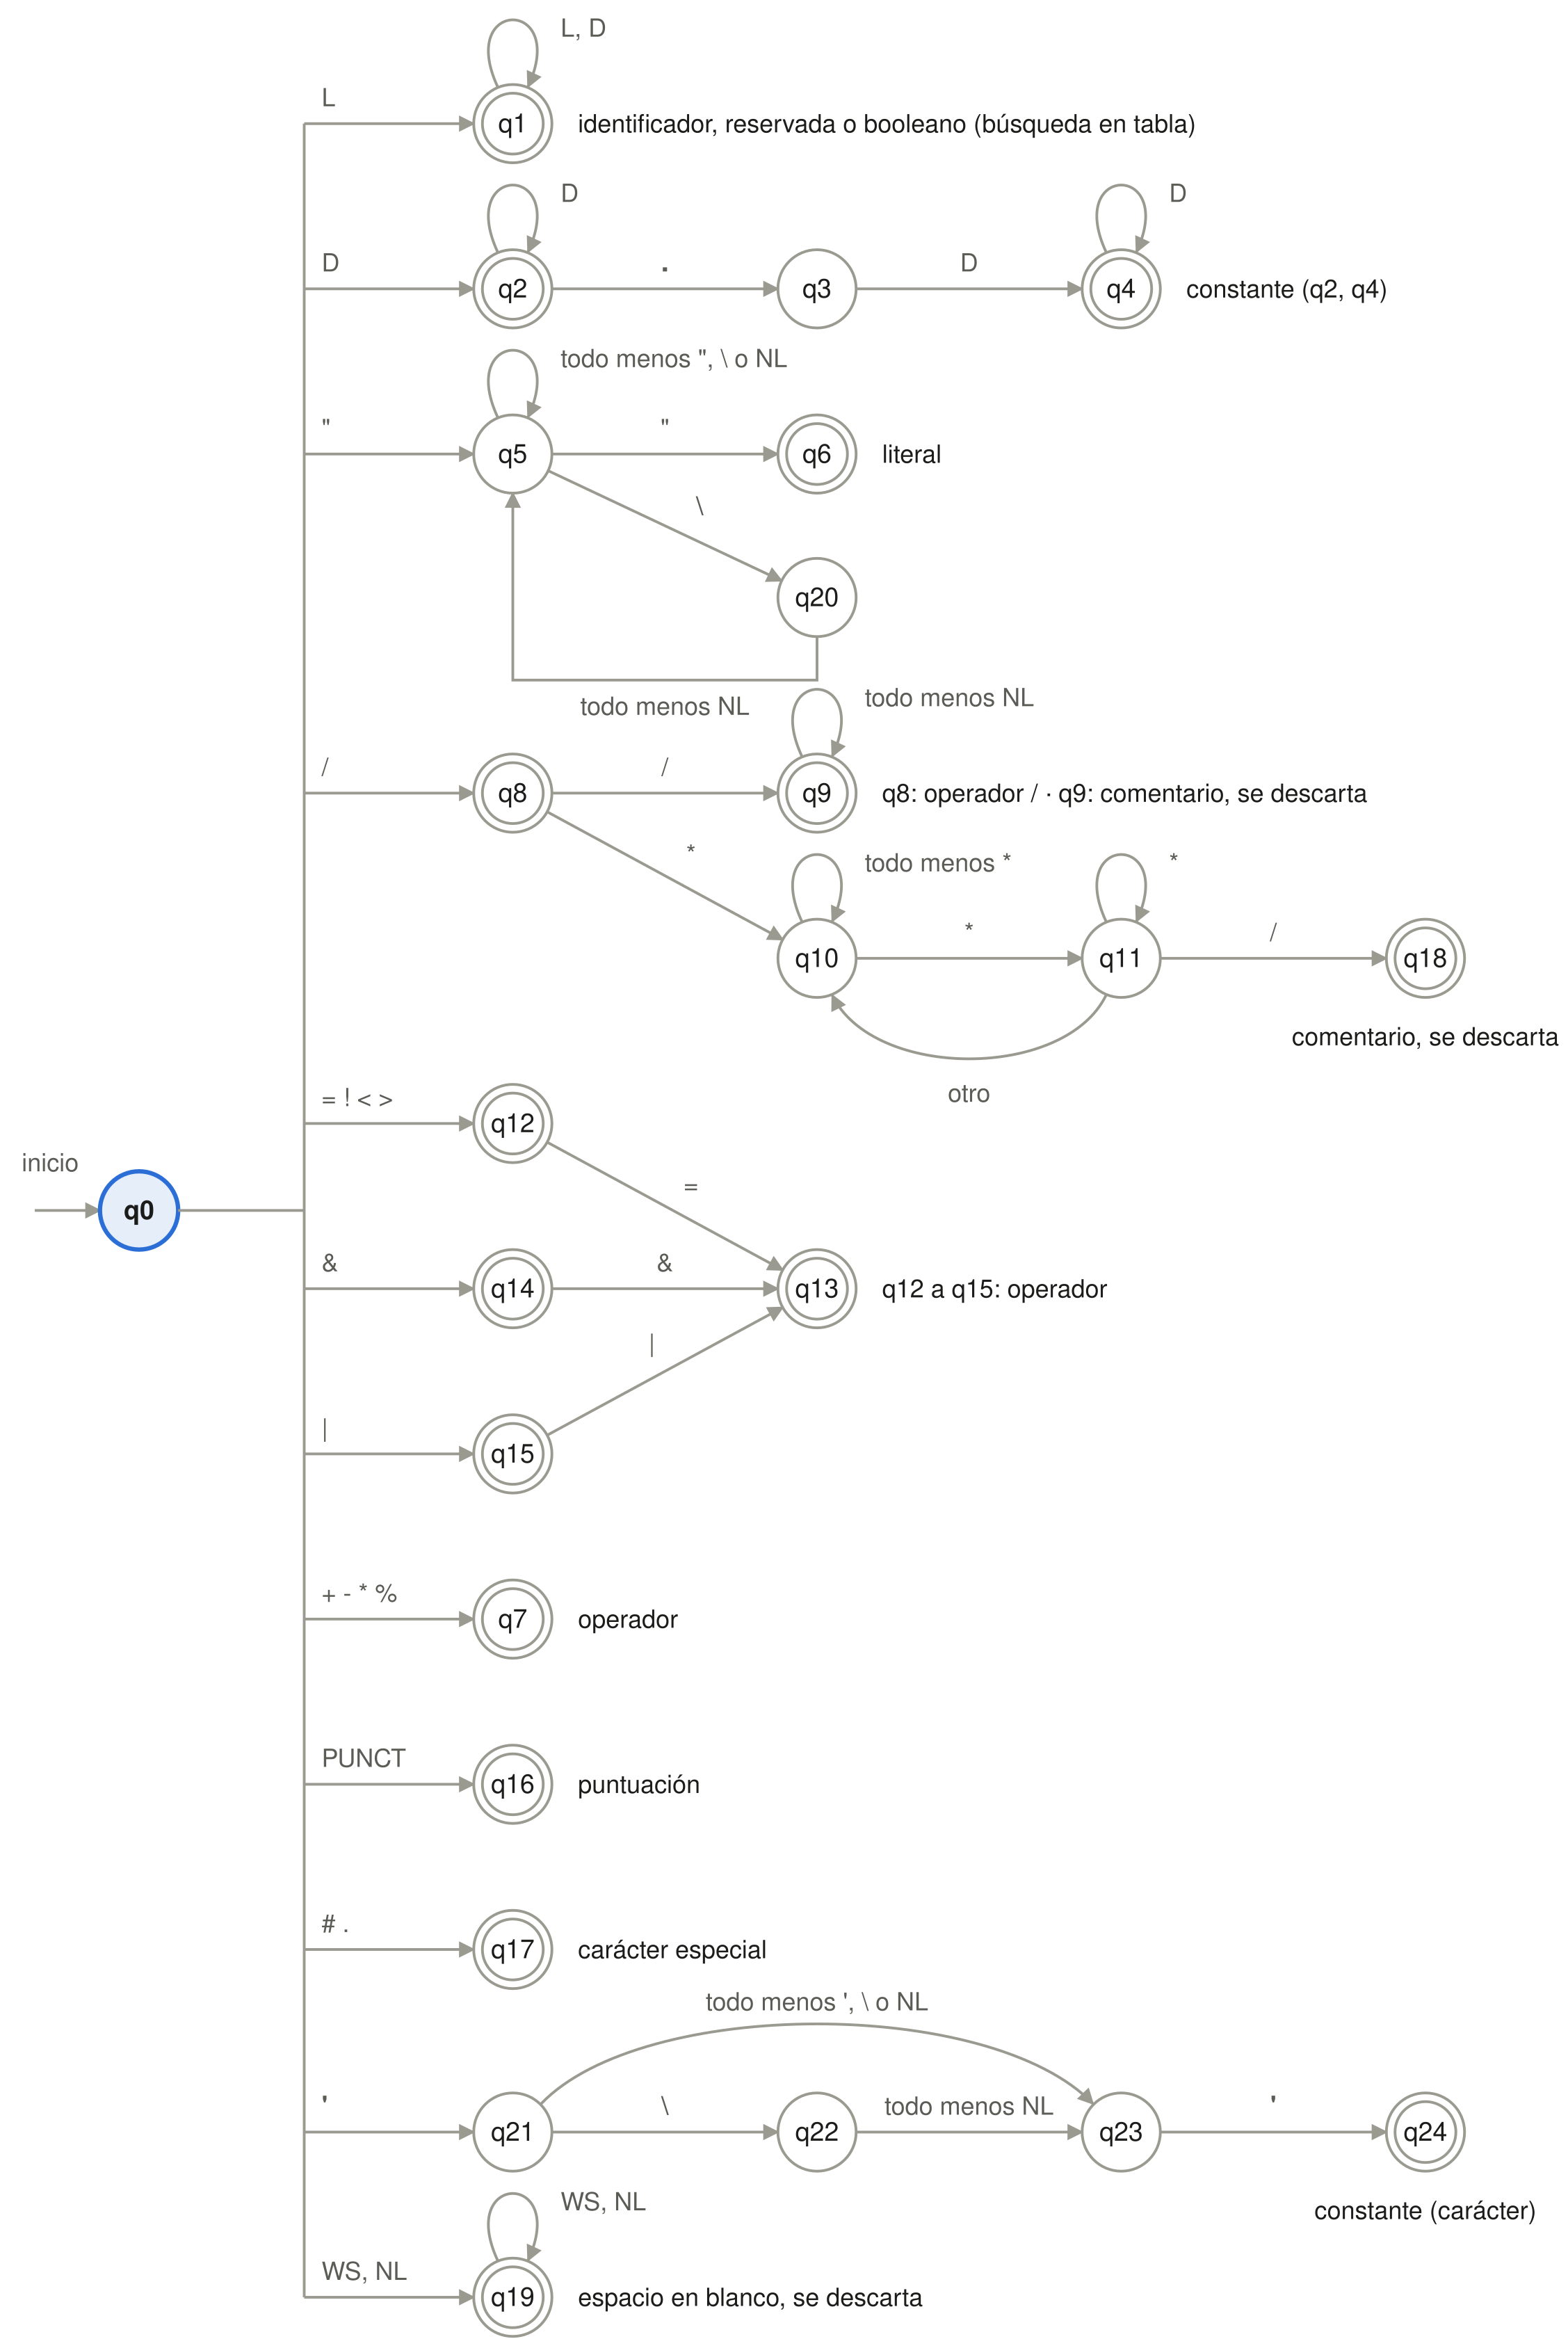
\includegraphics[width=0.95\textwidth]{afd.png}
    \caption{AFD del lexer · 25 estados, 16 finales}
\end{figure}

Cada clase de token tiene su propia fila, así que el estado final donde se detiene el escaneo fija la clase del lexema.

Algunos estados correspondientes a operadores presentan el mismo comportamiento respecto a las clases de entrada, por lo que pueden representarse mediante un mismo estado. Por ejemplo, los operadores \cd{=}, \cd{!}, \cd{<} y \cd{>} comparten un estado intermedio, ya que pueden finalizar individualmente o continuar con \cd{=} para formar un operador de dos caracteres. Por eso \cd{= ! < >} comparten $q_{12}$ y todos los operadores de dos caracteres terminan en $q_{13}$. $q_{14}$ y $q_{15}$ no se fusionan, porque $q_{14}$ avanza con \cd{\&} y $q_{15}$ con \cd{\textbar}.

Dos caracteres van en la misma columna si se comportan igual en todos los estados. Así, las 128 columnas de ASCII se reducen a 18. Esta agrupación evita definir una columna independiente para cada carácter ASCII. Por ejemplo, todas las letras se comportan de la misma manera en las transiciones asociadas a identificadores, por lo que se agrupan en la clase \cd{L}.

\begin{center}
\small
\begin{tabular}{@{}l l @{\hspace{1cm}} l l@{}}
\toprule
\textbf{Clase} & \textbf{Caracteres} & \textbf{Clase} & \textbf{Caracteres} \\
\midrule
\cd{L}      & \cd{a--z}, \cd{A--Z}, \cd{\_} & \cd{AMP}   & \cd{\&} \\
\cd{D}      & \cd{0--9}                     & \cd{BAR}   & \cd{\textbar} \\
\cd{DOT}    & \cd{.}                        & \cd{ARITH} & \cd{+ - \%} \\
\cd{QUOTE}  & \cd{"}                        & \cd{PUNCT} & \cd{( ) \{ \} [ ] ; ,} \\
\cd{APOS}   & \cd{\textquotesingle}         & \cd{HASH}  & \cd{\#} \\
\cd{BSLASH} & \cd{\textbackslash}           & \cd{WS}    & espacio, tabulador, retorno de carro \\
\cd{SLASH}  & \cd{/}                        & \cd{NL}    & salto de línea \\
\cd{STAR}   & \cd{*}                        & \cd{OTHER} & cualquier otro carácter \\
\cd{EQ}     & \cd{=}                        &            & \\
\cd{REL}    & \cd{! < >}                    &            & \\
\bottomrule
\end{tabular}
\end{center}

\textbf{Tabla de transiciones} $\delta(\text{estado}, \text{clase})$; un guion significa que no hay movimiento:

\begin{table}[H]
\centering
\resizebox{\textwidth}{!}{%
\begin{tabular}{@{}l *{18}{c}@{}}
\toprule
\textbf{STATE} & L & D & DOT & QUOTE & APOS & BSLASH & SLASH & STAR & EQ & REL & AMP & BAR & ARITH & PUNCT & HASH & WS & NL & OTHER \\
\midrule
$q_{0}$ & $q_{1}$ & $q_{2}$ & $q_{17}$ & $q_{5}$ & $q_{21}$ & -- & $q_{8}$ & $q_{7}$ & $q_{12}$ & $q_{12}$ & $q_{14}$ & $q_{15}$ & $q_{7}$ & $q_{16}$ & $q_{17}$ & $q_{19}$ & $q_{19}$ & -- \\
$q_{1}$ & $q_{1}$ & $q_{1}$ & -- & -- & -- & -- & -- & -- & -- & -- & -- & -- & -- & -- & -- & -- & -- & -- \\
$q_{2}$ & -- & $q_{2}$ & $q_{3}$ & -- & -- & -- & -- & -- & -- & -- & -- & -- & -- & -- & -- & -- & -- & -- \\
$q_{3}$ & -- & $q_{4}$ & -- & -- & -- & -- & -- & -- & -- & -- & -- & -- & -- & -- & -- & -- & -- & -- \\
$q_{4}$ & -- & $q_{4}$ & -- & -- & -- & -- & -- & -- & -- & -- & -- & -- & -- & -- & -- & -- & -- & -- \\
$q_{5}$ & $q_{5}$ & $q_{5}$ & $q_{5}$ & $q_{6}$ & $q_{5}$ & $q_{20}$ & $q_{5}$ & $q_{5}$ & $q_{5}$ & $q_{5}$ & $q_{5}$ & $q_{5}$ & $q_{5}$ & $q_{5}$ & $q_{5}$ & $q_{5}$ & -- & $q_{5}$ \\
$q_{6}$ & -- & -- & -- & -- & -- & -- & -- & -- & -- & -- & -- & -- & -- & -- & -- & -- & -- & -- \\
$q_{7}$ & -- & -- & -- & -- & -- & -- & -- & -- & -- & -- & -- & -- & -- & -- & -- & -- & -- & -- \\
$q_{8}$ & -- & -- & -- & -- & -- & -- & $q_{9}$ & $q_{10}$ & -- & -- & -- & -- & -- & -- & -- & -- & -- & -- \\
$q_{9}$ & $q_{9}$ & $q_{9}$ & $q_{9}$ & $q_{9}$ & $q_{9}$ & $q_{9}$ & $q_{9}$ & $q_{9}$ & $q_{9}$ & $q_{9}$ & $q_{9}$ & $q_{9}$ & $q_{9}$ & $q_{9}$ & $q_{9}$ & $q_{9}$ & -- & $q_{9}$ \\
$q_{10}$ & $q_{10}$ & $q_{10}$ & $q_{10}$ & $q_{10}$ & $q_{10}$ & $q_{10}$ & $q_{10}$ & $q_{11}$ & $q_{10}$ & $q_{10}$ & $q_{10}$ & $q_{10}$ & $q_{10}$ & $q_{10}$ & $q_{10}$ & $q_{10}$ & $q_{10}$ & $q_{10}$ \\
$q_{11}$ & $q_{10}$ & $q_{10}$ & $q_{10}$ & $q_{10}$ & $q_{10}$ & $q_{10}$ & $q_{18}$ & $q_{11}$ & $q_{10}$ & $q_{10}$ & $q_{10}$ & $q_{10}$ & $q_{10}$ & $q_{10}$ & $q_{10}$ & $q_{10}$ & $q_{10}$ & $q_{10}$ \\
$q_{12}$ & -- & -- & -- & -- & -- & -- & -- & -- & $q_{13}$ & -- & -- & -- & -- & -- & -- & -- & -- & -- \\
$q_{13}$ & -- & -- & -- & -- & -- & -- & -- & -- & -- & -- & -- & -- & -- & -- & -- & -- & -- & -- \\
$q_{14}$ & -- & -- & -- & -- & -- & -- & -- & -- & -- & -- & $q_{13}$ & -- & -- & -- & -- & -- & -- & -- \\
$q_{15}$ & -- & -- & -- & -- & -- & -- & -- & -- & -- & -- & -- & $q_{13}$ & -- & -- & -- & -- & -- & -- \\
$q_{16}$ & -- & -- & -- & -- & -- & -- & -- & -- & -- & -- & -- & -- & -- & -- & -- & -- & -- & -- \\
$q_{17}$ & -- & -- & -- & -- & -- & -- & -- & -- & -- & -- & -- & -- & -- & -- & -- & -- & -- & -- \\
$q_{18}$ & -- & -- & -- & -- & -- & -- & -- & -- & -- & -- & -- & -- & -- & -- & -- & -- & -- & -- \\
$q_{19}$ & -- & -- & -- & -- & -- & -- & -- & -- & -- & -- & -- & -- & -- & -- & -- & $q_{19}$ & $q_{19}$ & -- \\
$q_{20}$ & $q_{5}$ & $q_{5}$ & $q_{5}$ & $q_{5}$ & $q_{5}$ & $q_{5}$ & $q_{5}$ & $q_{5}$ & $q_{5}$ & $q_{5}$ & $q_{5}$ & $q_{5}$ & $q_{5}$ & $q_{5}$ & $q_{5}$ & $q_{5}$ & -- & $q_{5}$ \\
$q_{21}$ & $q_{23}$ & $q_{23}$ & $q_{23}$ & $q_{23}$ & -- & $q_{22}$ & $q_{23}$ & $q_{23}$ & $q_{23}$ & $q_{23}$ & $q_{23}$ & $q_{23}$ & $q_{23}$ & $q_{23}$ & $q_{23}$ & $q_{23}$ & -- & $q_{23}$ \\
$q_{22}$ & $q_{23}$ & $q_{23}$ & $q_{23}$ & $q_{23}$ & $q_{23}$ & $q_{23}$ & $q_{23}$ & $q_{23}$ & $q_{23}$ & $q_{23}$ & $q_{23}$ & $q_{23}$ & $q_{23}$ & $q_{23}$ & $q_{23}$ & $q_{23}$ & -- & $q_{23}$ \\
$q_{23}$ & -- & -- & -- & -- & $q_{24}$ & -- & -- & -- & -- & -- & -- & -- & -- & -- & -- & -- & -- & -- \\
$q_{24}$ & -- & -- & -- & -- & -- & -- & -- & -- & -- & -- & -- & -- & -- & -- & -- & -- & -- & -- \\
\bottomrule
\end{tabular}}
\caption{Tabla de transiciones del AFD (25 estados $\times$ 18 clases)}
\end{table}

\textbf{Estados finales} ($q_0$, $q_3$, $q_5$, $q_{10}$, $q_{11}$ y $q_{20}$ a $q_{23}$ no son finales):

\begin{center}
\small
\begin{tabularx}{\textwidth}{@{}l p{4.6cm} X@{}}
\toprule
\textbf{Estado final} & \textbf{Lexemas que termina} & \textbf{Regresa} \\
\midrule
$q_1$ & palabras & el \cd{TokenType} de la tabla de búsqueda; si no está, \cd{ID} \\
$q_2$ & \cd{10} & \cd{INT\_CONST} \\
$q_4$ & \cd{3.14} & \cd{FLOAT\_CONST} \\
$q_{24}$ & \cd{\textquotesingle a\textquotesingle}, \cd{\textquotesingle\textbackslash n\textquotesingle} & \cd{CHAR\_CONST} \\
$q_6$ & \cd{"..."} & \cd{STRING} \\
$q_7, q_8, q_{12}, q_{13}, q_{14}, q_{15}$ & \cd{+ - * \% / = ! < > == != <= >= \& \&\& \textbar\ \textbar\textbar} & el operador según el lexema (\cd{PLUS}, \cd{EQ}, \cd{AND}\ldots) \\
$q_{16}$ & \cd{( ) \{ \} [ ] ; ,} & la puntuación según el lexema (\cd{LPAREN}, \cd{SEMI}\ldots) \\
$q_{17}$ & \cd{\# .} & \cd{HASH} o \cd{DOT} \\
$q_9, q_{18}$ & \cd{// ...}, \cd{/* ... */} & comentario, se descarta \\
$q_{19}$ & espacios, tabuladores, saltos de línea & espacio en blanco, se descarta \\
\bottomrule
\end{tabularx}
\end{center}

\subsection{Consideraciones en el proceso de escaneo}

Un error léxico ocurre cuando el escaneo se detiene sin haber pasado por un estado final. Para el AFD construido, los principales casos en los que el escaneo puede detenerse sin obtener un token válido son en los siguientes estados:

\begin{center}
\footnotesize
\begin{tabularx}{\textwidth}{@{}p{2.4cm} p{3.6cm} p{4.3cm} X@{}}
\toprule
\textbf{Estado donde se atora} & \textbf{Qué significa} & \textbf{Mensaje} & \textbf{Recuperación} \\
\midrule
$q_0$ & carácter que no inicia ningún token, como \cd{@} o \cd{\textbackslash} & \cd{Lexical error 1:5: unexpected character \textquotesingle @\textquotesingle} & saltar ese carácter \\
$q_5$ o $q_{20}$ & cadena sin cerrar en la misma línea & \cd{Lexical error 2:8: unterminated string literal} & saltar al final de la línea \\
$q_{21}$, $q_{22}$ o $q_{23}$ & constante de carácter mal formada: \cd{\textquotesingle\textquotesingle}, \cd{\textquotesingle ab\textquotesingle} o sin cerrar & \cd{Lexical error 3:10: malformed character constant} & saltar hasta la siguiente \cd{\textquotesingle} de la línea, o al final de la línea \\
$q_{10}$ o $q_{11}$, al final de la entrada & comentario de bloque sin cerrar (regla 4) & \cd{Lexical error 4:1: unterminated comment} & dejar de escanear \\
\bottomrule
\end{tabularx}
\end{center}

En $q_3$ no hay error: \cd{5.} siempre tiene antes el estado final $q_2$, así que se emite \cd{5} y se vuelve a escanear desde \cd{.}. La recuperación del carácter salta hasta la siguiente comilla para que \cd{\textquotesingle ab\textquotesingle} no se convierta en un identificador falso más otro error.

%=====================================================================
\section{Diagramas del proceso del lexer}
El diagrama de flujo muestra cómo los errores y los elementos descartados regresan al inicio del ciclo sin agregar tokens. La ejecución del Lexer se realiza en 5 etapas mostradas en el siguiente gráfico.

\begin{figure}[H]
    \centering
    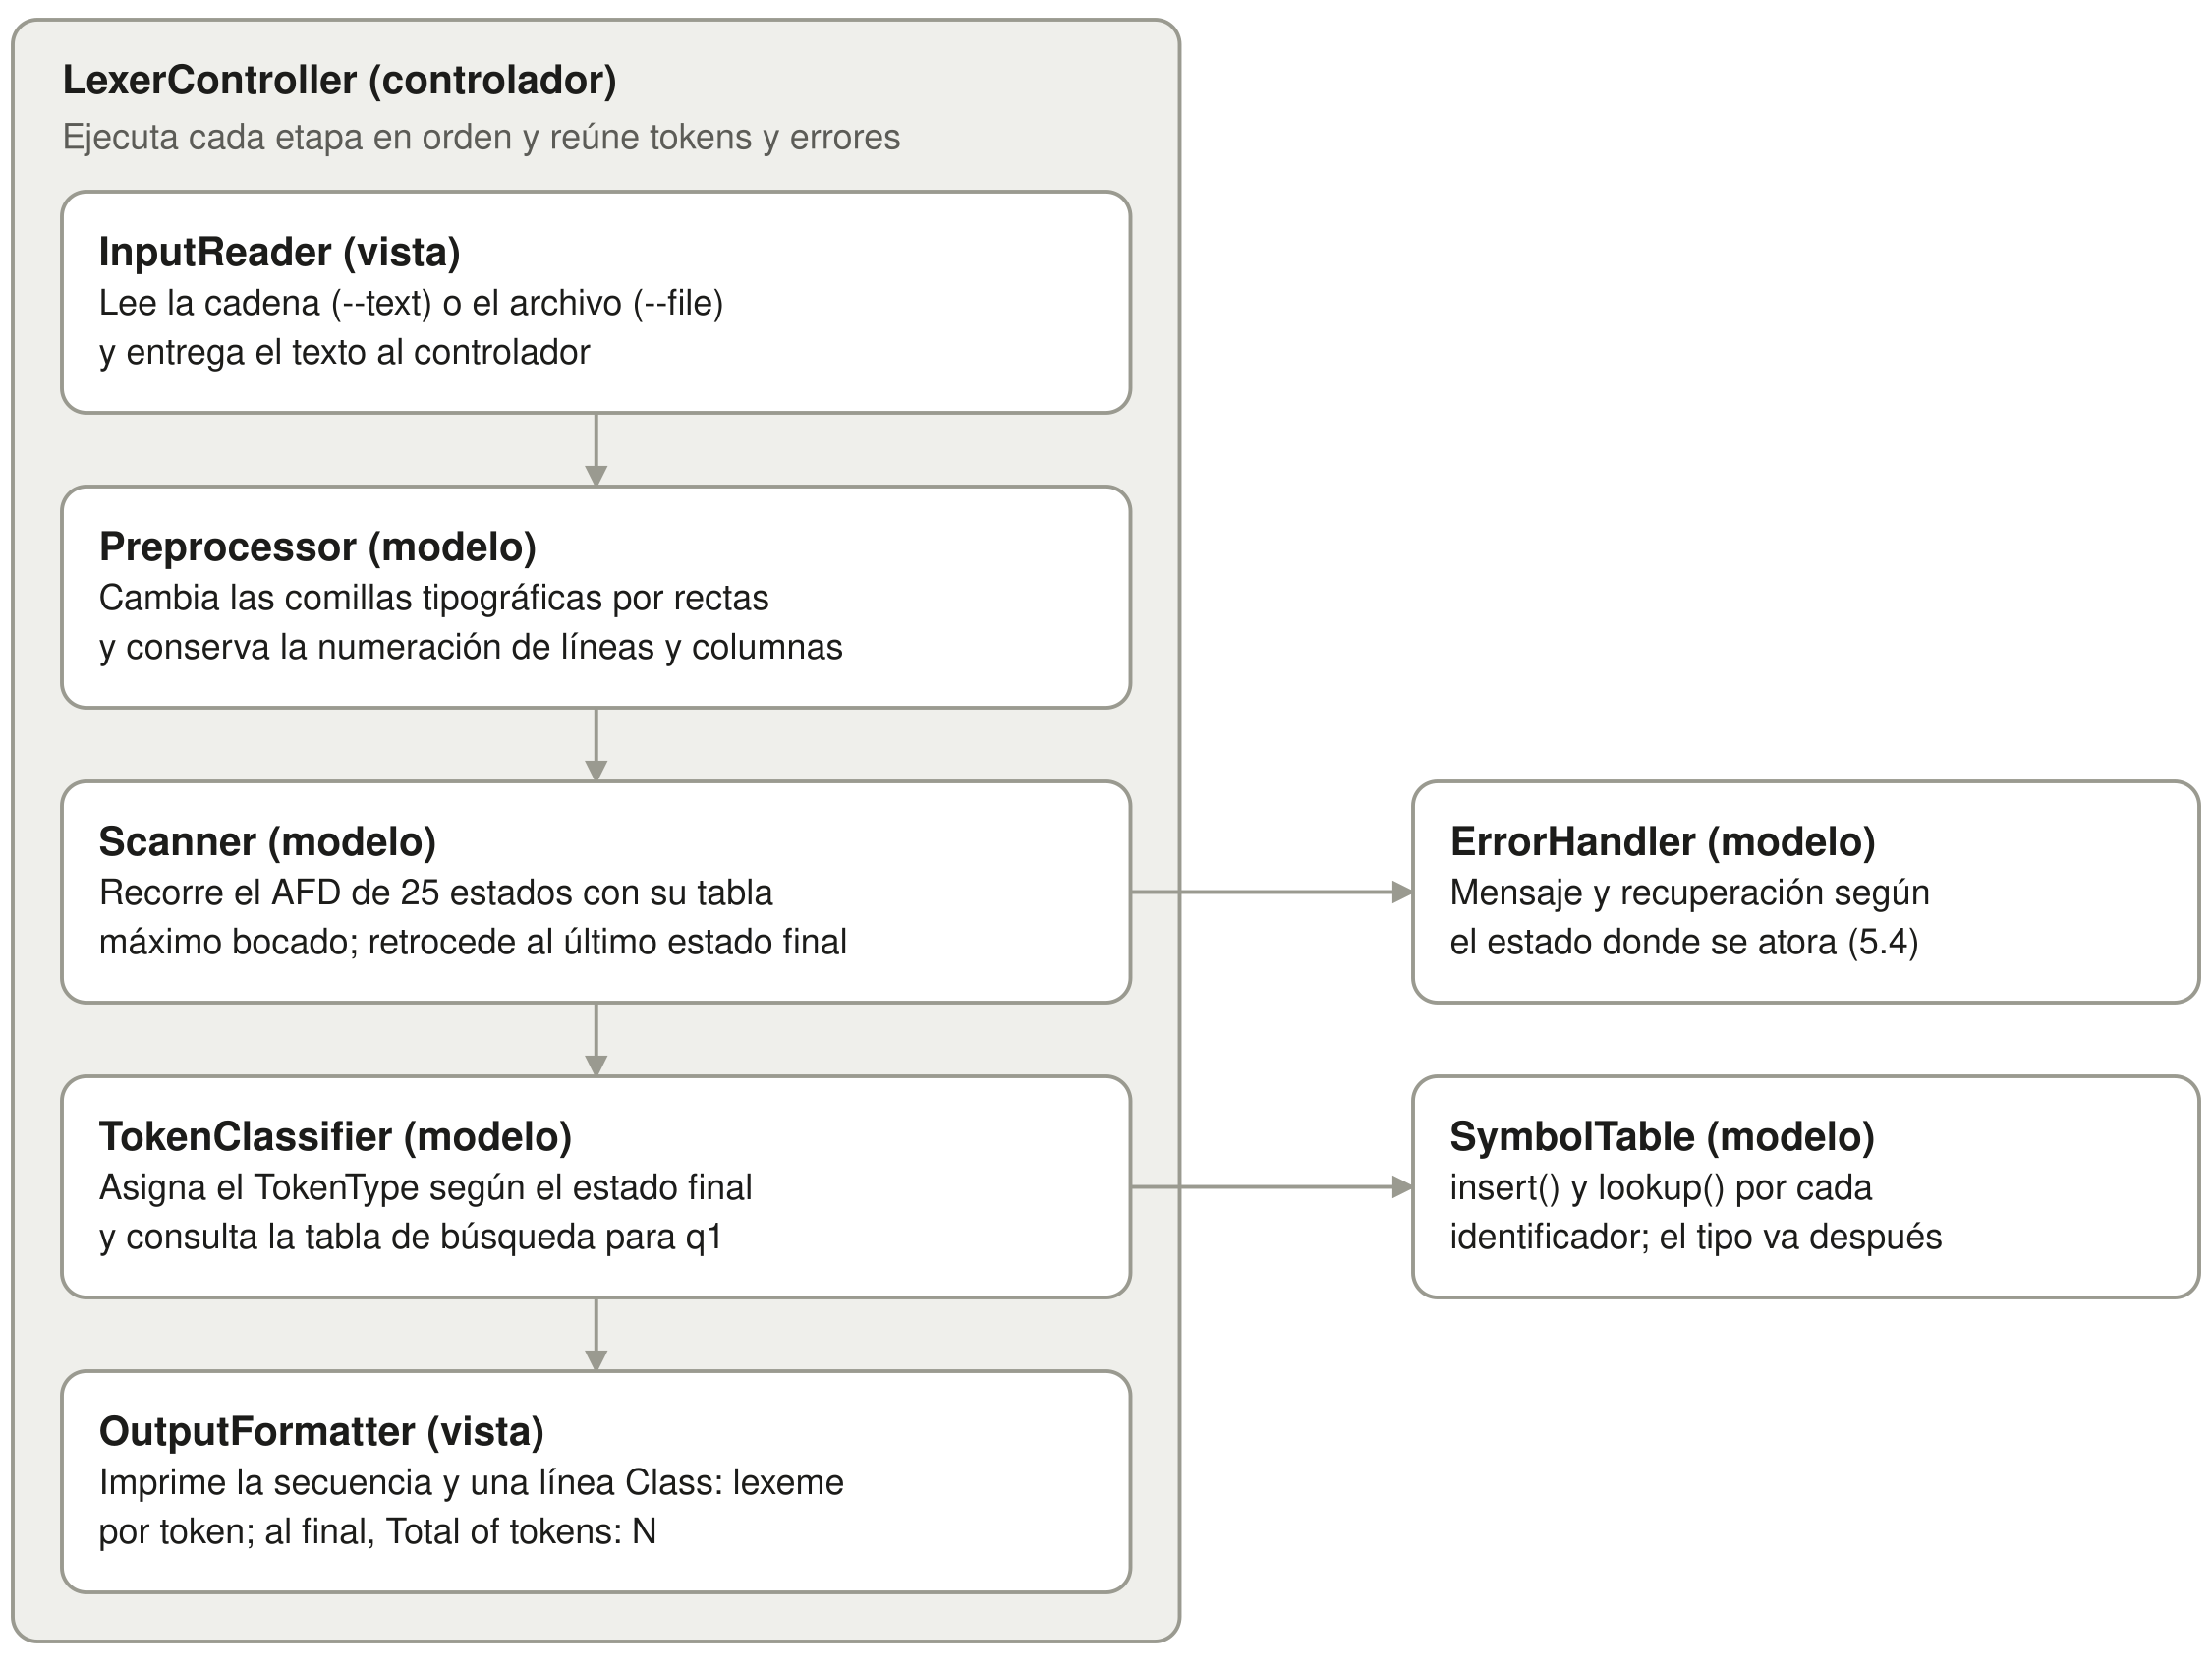
\includegraphics[width=0.85\textwidth]{etapas.png}
    \caption{Etapas del lexer · 5 etapas}
\end{figure}

\subsection{Ciclo de escaneo}

En la siguiente imagen se muestra un diagrama de flujo del proceso scan del Lexer.

\begin{figure}[H]
    \centering
    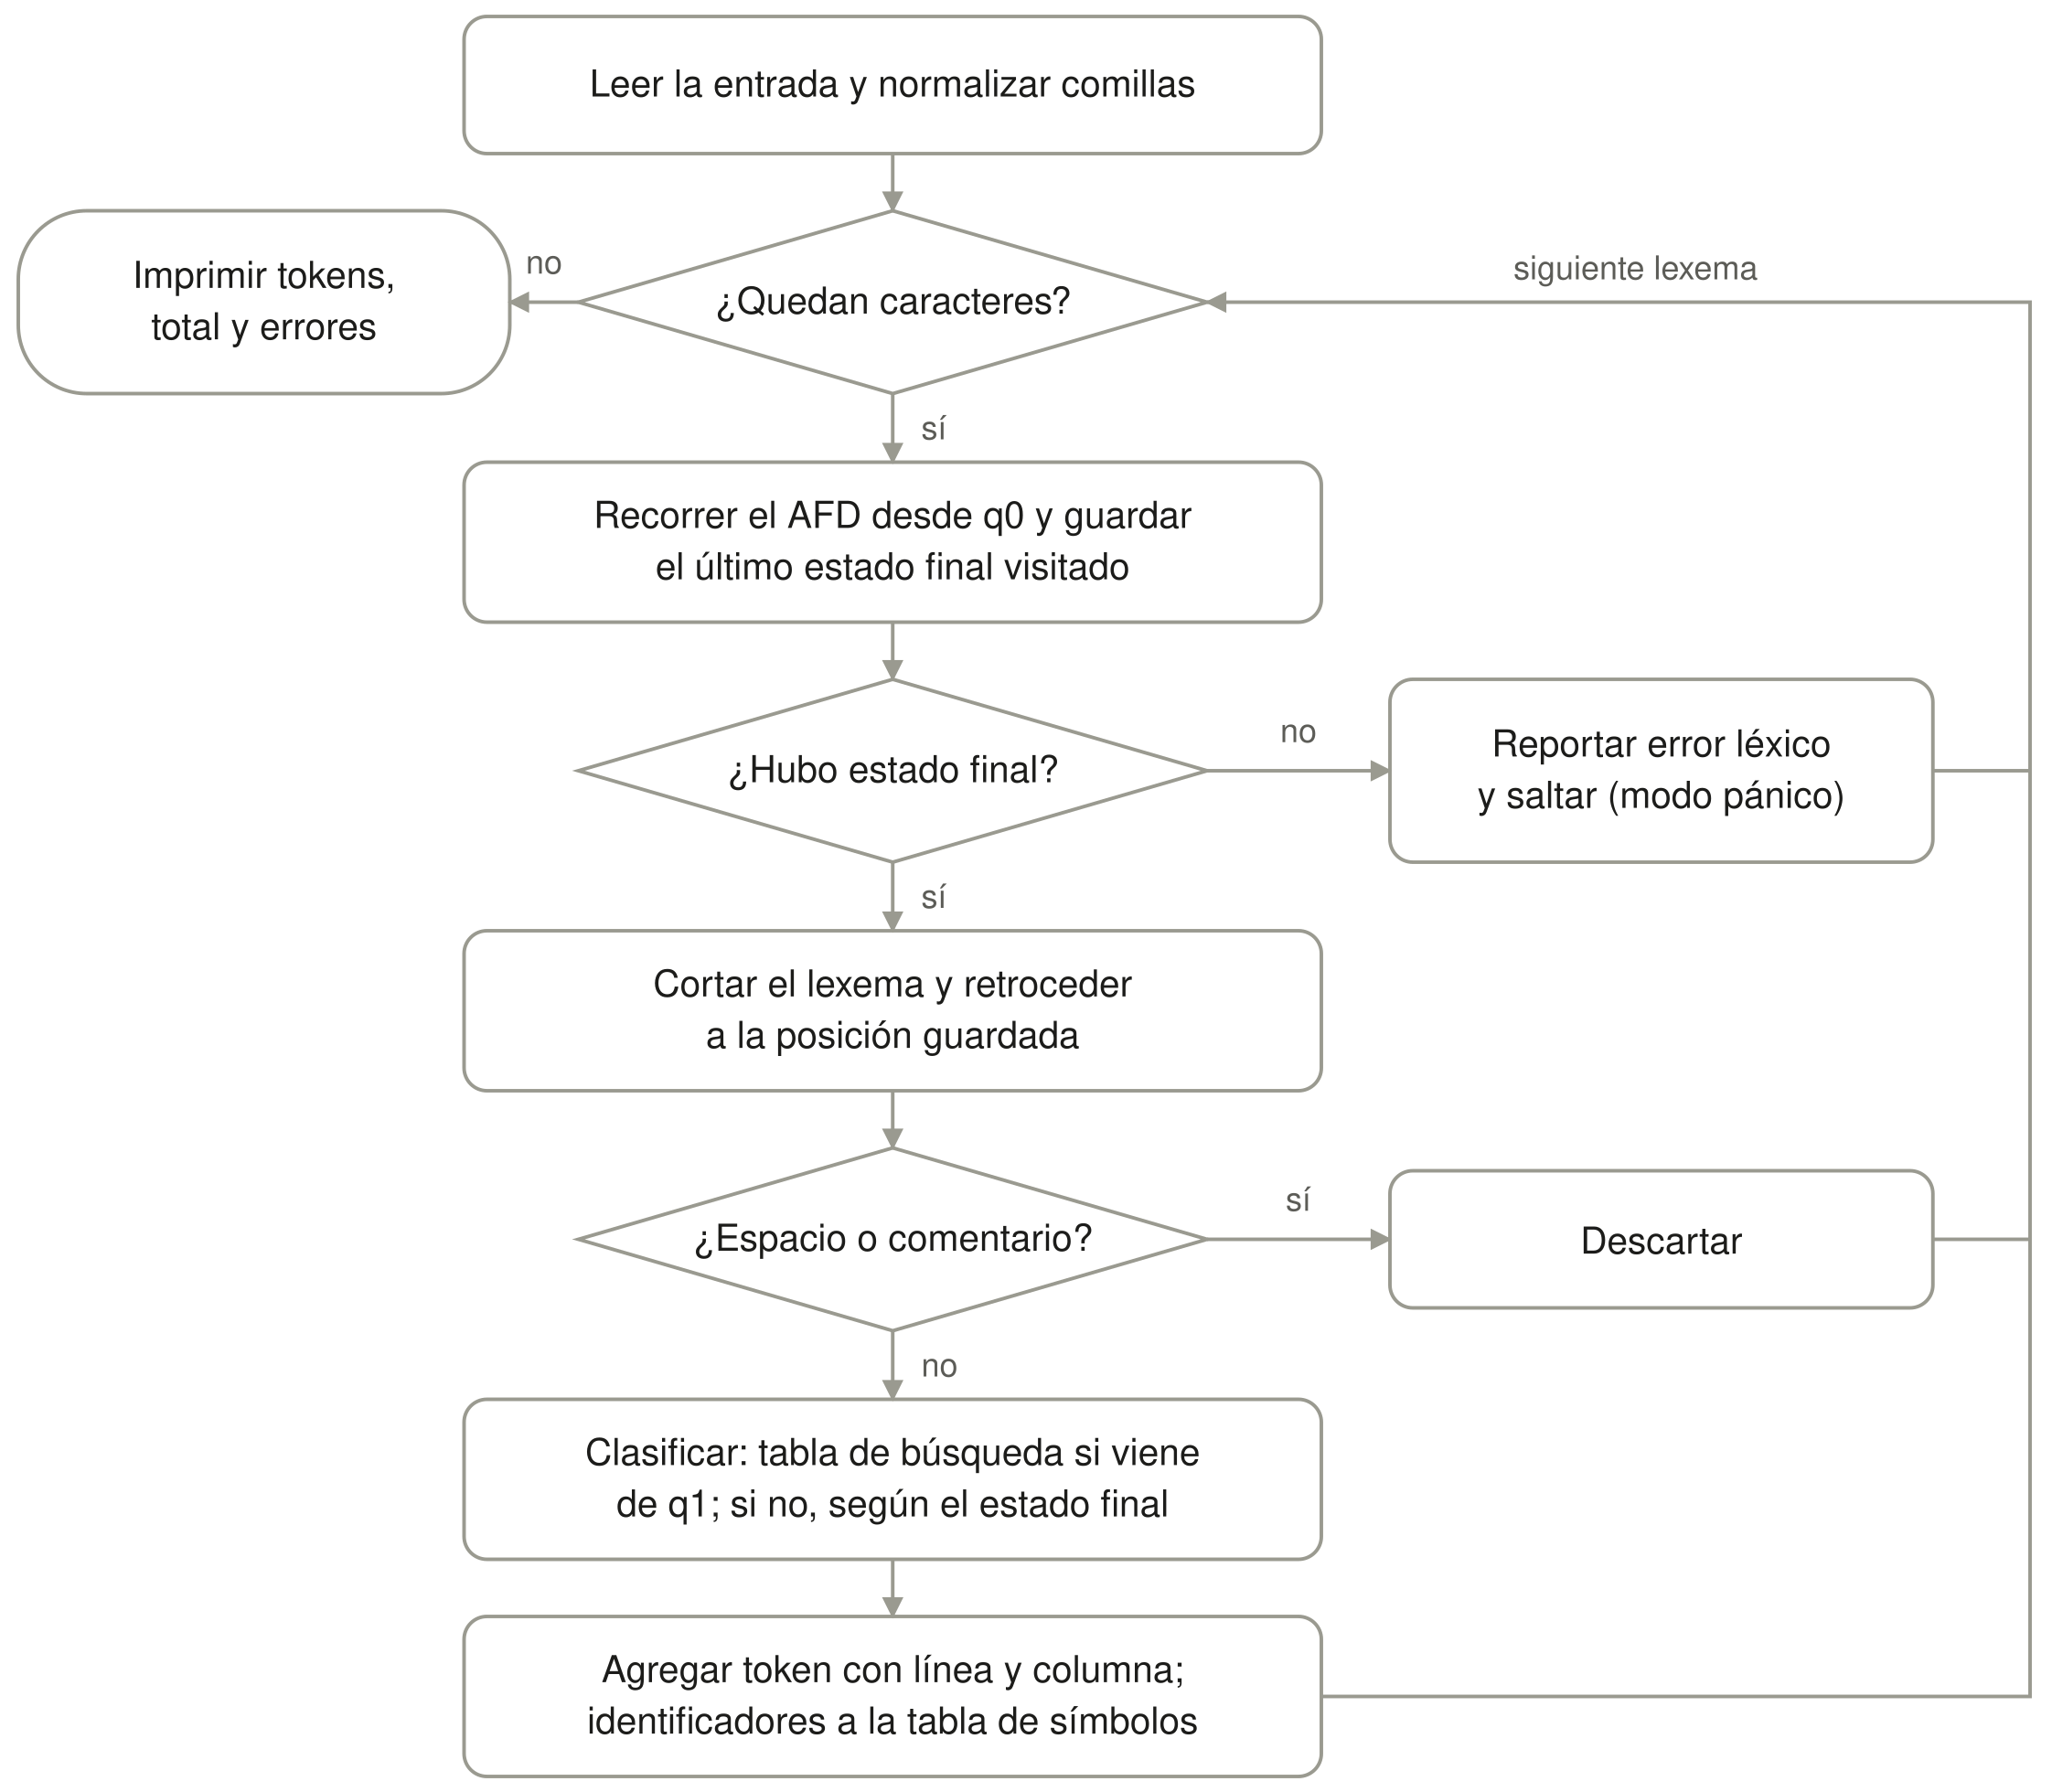
\includegraphics[width=0.85\textwidth]{flujo-escaneo.png}
    \caption{Diagrama de flujo del escaneo}
\end{figure}

Cada vuelta del ciclo consume un lexema; los errores y los elementos descartados regresan al inicio sin agregar tokens.

La construcción de este diagrama se obtuvo a partir del pseudocódigo; if es un rombo de decisión, así mismo, cada grupo de instrucciones a una caja.

\begin{lstlisting}
while pos < len(text):
    state = q0; i = pos; lastFinal = none; lastEnd = pos
    while i < len(text):
        next = delta[state][classOf(text[i])]
        if next == none: break
        state = next; i = i + 1
        if state in FINAL: lastFinal = state; lastEnd = i
    if i == len(text) and state in {q10, q11}:
        errors.report(line, col, "unterminated comment"); break
    if lastFinal == none:
        errors.report(line, col, state); pos = recover(pos, state); continue
    lexeme = text[pos : lastEnd]
    kind = classify(lastFinal, lexeme)   # aquí se consulta la tabla de búsqueda
    if kind not in {WHITESPACE, COMMENT}:
        tokens.add(kind, lexeme, line, col)
    advanceLineCol(lexeme); pos = lastEnd
\end{lstlisting}

%=====================================================================
\section{CFG}

A continuacón se presenta la Gramática Libre de Contexto $G_0 = (N, T, P, S)$ para la declaración, con $N = \{\text{Decl}, \text{Type}, \text{Value}\}$, $T = \{\texttt{int}, \texttt{float}, \texttt{char}, \texttt{id}, \texttt{num}, \texttt{=}, \texttt{;}\}$ y $S = \text{Decl}$.

\begin{align*}
&1.\ \text{Decl} \rightarrow \text{Type}\ \texttt{id}\ \texttt{;} \\
&2.\ \text{Decl} \rightarrow \text{Type}\ \texttt{id}\ \texttt{=}\ \text{Value}\ \texttt{;} \\
&3.\ \text{Type} \rightarrow \texttt{int} \mid \texttt{float} \mid \texttt{char} \\
&4.\ \text{Value} \rightarrow \texttt{num} \mid \texttt{id}
\end{align*}

Se eligió una declaración de variable porque permite mostrar un caso de producciones con prefijo común con el fin de aplicar producciones por left factoring.

Se tomó la secuencia de tokens \cd{int id = num ;} y se escribió una producción por cada forma de la declaración sin valor y con valor. Los terminales son tokens del siguiente catálogo:

\begin{center}
\small
\begin{tabular}{@{}l l@{}}
\toprule
\textbf{Terminal} & \textbf{TokenType} \\
\midrule
\cd{int}, \cd{float}, \cd{char} & \cd{INT}, \cd{FLOAT}, \cd{CHAR} \\
\cd{id}  & \cd{ID} \\
\cd{num} & \cd{INT\_CONST} \\
\cd{=}   & \cd{ASSIGN} \\
\cd{;}   & \cd{SEMI} \\
\bottomrule
\end{tabular}
\end{center}

Existe una consideración para la generación de LL(1). Las producciones 1 y 2 comparten el prefijo \cd{Type id}. Después de leer \cd{int a}, otro tippo de analizador no tendría esta consideración, por consecuencia, no sabría cuál aplicar, por lo tanto, en una tabla LL(1) ambas caerían en la celda $[\text{Decl}, \texttt{int}]$.


%=====================================================================
\section{Left factoring}

Se factorizó el prefijo común de $G_0$ y se verificó que el resultado, $G_1$, es LL(1). Así mismo, se buscó el prefijo común más largo de las dos producciones de Decl: $\alpha = \text{Type}\ \texttt{id}$. Lo que sigue en cada una es $\beta_1 = \texttt{;}$ y $\beta_2 = \texttt{=}\ \text{Value}\ \texttt{;}$. Se aplicó la regla vista en clase.

\[A \to \alpha\beta_1 \mid \alpha\beta_2 \quad\Longrightarrow\quad A \to \alpha A', \qquad A' \to \beta_1 \mid \beta_2\]

\begin{align*}
&1.\ \text{Decl} \rightarrow \text{Type}\ \texttt{id}\ \text{Decl}' \\
&2.\ \text{Decl}' \rightarrow \texttt{;} \mid \texttt{=}\ \text{Value}\ \texttt{;} \\
&3.\ \text{Type} \rightarrow \texttt{int} \mid \texttt{float} \mid \texttt{char} \\
&4.\ \text{Value} \rightarrow \texttt{num} \mid \texttt{id}
\end{align*}

La gramática resultante no presenta left factoring y elimina el prefijo común de las producciones de Decl. Posteriormente se verificó mediante FIRST, FOLLOW y la tabla predictiva que no presenta conflictos para este ejemplo.

\subsection{FIRST, FOLLOW, tabla LL(1) y traza.}

En la siguiente tabla se muestra el resultado de las operaciones First y Follow para la gramática.

\begin{center}
\small
\begin{tabular}{@{}l l l@{}}
\toprule
\textbf{No terminal} & \textbf{FIRST} & \textbf{FOLLOW} \\
\midrule
Decl & $\{\texttt{int}, \texttt{float}, \texttt{char}\}$ & $\{\$\}$ \\
Decl$'$ & $\{\texttt{;}, \texttt{=}\}$ & $\{\$\}$ \\
Type & $\{\texttt{int}, \texttt{float}, \texttt{char}\}$ & $\{\texttt{id}\}$ \\
Value & $\{\texttt{num}, \texttt{id}\}$ & $\{\texttt{;}\}$ \\
\bottomrule
\end{tabular}
\end{center}

\begin{table}[H]
\centering
\scriptsize
\renewcommand{\arraystretch}{1.3}
\resizebox{\textwidth}{!}{%
\begin{tabular}{@{}l c c c c c c c c@{}}
\toprule
 & \texttt{int} & \texttt{float} & \texttt{char} & \texttt{id} & \texttt{num} & \texttt{=} & \texttt{;} & \texttt{\$} \\
\midrule
Decl  & $\text{Decl}\to\text{Type}\ \texttt{id}\ \text{Decl}'$ & $\text{Decl}\to\text{Type}\ \texttt{id}\ \text{Decl}'$ & $\text{Decl}\to\text{Type}\ \texttt{id}\ \text{Decl}'$ & & & & & \\
Decl$'$ & & & & & & $\text{Decl}'\to\texttt{=}\ \text{Value}\ \texttt{;}$ & $\text{Decl}'\to\texttt{;}$ & \\
Type  & $\text{Type}\to\texttt{int}$ & $\text{Type}\to\texttt{float}$ & $\text{Type}\to\texttt{char}$ & & & & & \\
Value & & & & $\text{Value}\to\texttt{id}$ & $\text{Value}\to\texttt{num}$ & & & \\
\bottomrule
\end{tabular}}
\end{table}
Cada celda tiene a lo más una producción, así que $G_1$ es LL(1). Traza de \cd{int id = num ;}, con el tope de la pila a la derecha como en clase:

\begin{center}
\small
\begin{tabular}{@{}r l l l@{}}
\toprule
\textbf{Paso} & \textbf{Pila} & \textbf{Entrada} & \textbf{Acción} \\
\midrule
1  & \texttt{\$ Decl}            & \texttt{int id = num ; \$} & $\text{Decl} \to \text{Type}\ \texttt{id}\ \text{Decl}'$ \\
2  & \texttt{\$ Decl' id Type}   & \texttt{int id = num ; \$} & $\text{Type} \to \texttt{int}$ \\
3  & \texttt{\$ Decl' id int}    & \texttt{int id = num ; \$} & match \texttt{int} \\
4  & \texttt{\$ Decl' id}        & \texttt{id = num ; \$}     & match \texttt{id} \\
5  & \texttt{\$ Decl'}           & \texttt{= num ; \$}        & $\text{Decl}' \to \texttt{=}\ \text{Value}\ \texttt{;}$ \\
6  & \texttt{\$ ; Value =}       & \texttt{= num ; \$}        & match \texttt{=} \\
7  & \texttt{\$ ; Value}         & \texttt{num ; \$}          & $\text{Value} \to \texttt{num}$ \\
8  & \texttt{\$ ; num}           & \texttt{num ; \$}          & match \texttt{num} \\
9  & \texttt{\$ ;}               & \texttt{; \$}              & match \texttt{;} \\
10 & \texttt{\$}                 & \texttt{\$}                & éxito \\
\bottomrule
\end{tabular}
\end{center}

\begin{figure}[H]
    \centering
    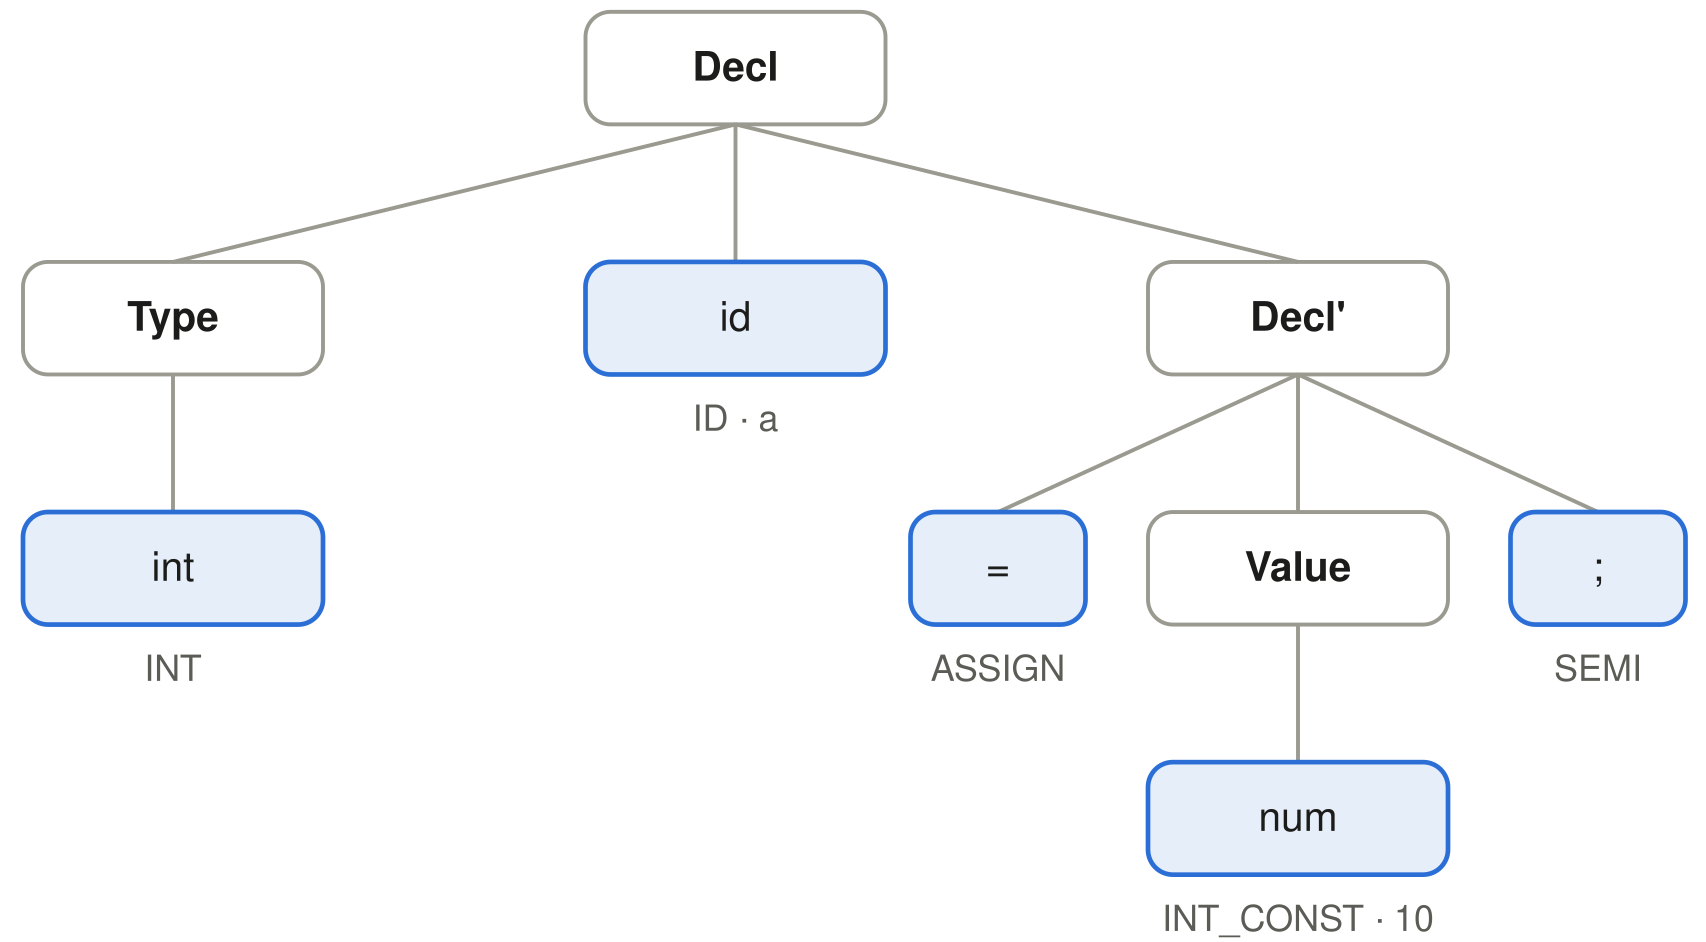
\includegraphics[width=0.85\textwidth]{arbol-sintactico.png}
    \caption{Árbol sintáctico de \texttt{int a = 10;} · gramática $G_1$}
\end{figure}

Las hojas del árbol son los tokens \cd{INT}, \cd{ID}, \cd{ASSIGN}, \cd{INT\_CONST} y \cd{SEMI}: exactamente la salida del lexer para T2.

%=====================================================================

\end{document}